%\documentclass[10pt,journal,compsoc]{IEEEtran}
%\ifCLASSOPTIONcompsoc
%  \usepackage[nocompress]{cite}
%\else
%  \usepackage{cite}
%\fi

\documentclass[letterpaper,journal,10pt]{IEEEtran}
\IEEEoverridecommandlockouts
% The preceding line is only needed to identify funding in the first footnote. If that is unneeded, please comment it out.
\usepackage{cite}
\usepackage{amsmath,amssymb,amsfonts,amsthm}
\usepackage[linesnumbered,ruled,vlined]{algorithm2e}
\usepackage{algorithmic}
%\usepackage{algpseudocode}
%\usepackage{algorithmicx}
%\usepackage{algorithmic}
%\usepackage{algorithm}
\usepackage{graphicx}
\usepackage{textcomp}
\usepackage{xcolor}
\usepackage{epstopdf}
\usepackage{multicol}
\usepackage{multirow}
\usepackage{subfigure}
\usepackage{booktabs}

\usepackage{mathtools}
\usepackage{mathrsfs}
\usepackage{amsfonts}
\usepackage{bm}
\usepackage{cases}
\usepackage{array}
\usepackage{listings}
\usepackage{longtable}
\usepackage{indentfirst}
\usepackage{geometry}
\usepackage{float}
\usepackage{placeins}
%\usepackage{subfig}
\usepackage{threeparttable}
\usepackage{verbatim}
\usepackage{svg}
\usepackage{ragged2e}

\usepackage{tikz}
\usetikzlibrary{mindmap,trees,positioning,arrows.meta}
\usepackage{verbatim}
% CJK was inherited from an earlier draft but is not used by the English manuscript.
% Keeping it here made clean CI builds depend on a nonessential legacy package.
\usepackage{makecell}

\usepackage[hidelinks]{hyperref}
\hypersetup{colorlinks=true,
	allcolors=black,
	pdfstartview=Fit,
	breaklinks=true,
    urlcolor=blue}

\newtheorem{definition}{Definition}
\newtheorem{theorem}{Theorem}
\newtheorem{lemma}{Lemma}
\newtheorem{proposition}{Proposition}
\newtheorem{assumption}{Assumption}
\newtheorem{problem}{Problem}
\newtheorem{observation}{Observation}
\newtheorem{strategy}{Strategy}
\newtheorem{scenario}{Scenario}

\hyphenation{op-tical net-works semi-conduc-tor}
\geometry{letterpaper,scale=0.9}
\setlength{\textfloatsep}{7pt plus 1pt minus 2pt}
\setlength{\floatsep}{7pt plus 1pt minus 2pt}
\setlength{\intextsep}{7pt plus 1pt minus 2pt}
\renewcommand{\topfraction}{0.95}
\renewcommand{\bottomfraction}{0.95}
\renewcommand{\textfraction}{0.05}
\renewcommand{\floatpagefraction}{0.85}
\setcounter{topnumber}{3}
\setcounter{bottomnumber}{2}
\setcounter{totalnumber}{5}
\makeatletter
\setlength{\@fptop}{0pt}
\setlength{\@fpsep}{10pt plus 1pt minus 1pt}
\setlength{\@fpbot}{0pt plus 1fil}
\makeatother

\begin{document}

\title{KG-FedMARL: Knowledge-Guided Federated Multi-Agent Reinforcement Learning for Resilient Restoration of Power Cyber-Physical Systems\\
}
\author{
        Kai~Zhong,
        Zhibang~Yang,
        Siyang~Yu,
        Kenli~Li,~\IEEEmembership{Senior Member,~IEEE}
\IEEEcompsocitemizethanks
{
\IEEEcompsocthanksitem Kai Zhong and Kenli Li are with the College of Computer Science and Electronic Engineering, Hunan University, Changsha 410082, China.
\IEEEcompsocthanksitem Zhibang Yang is with the Hunan Province Key Laboratory of Industrial Internet Technology and Security, Changsha University, Changsha 410022, China.
\IEEEcompsocthanksitem Siyang Yu is with the College of Information Technology and Management, Hunan University of Finance and Economics, Changsha 410000, China.
\protect\\ E-mail: startkz@hnu.edu.cn, yangzhibang2006@126.com, yusiyang@hufe.edu.cn, lkl@hnu.edu.cn.
}%
\thanks{Manuscript received ****, 2026; revised ****, 2026.}
}

\markboth{IEEE TRANSACTIONS ON DEPENDABLE AND SECURE COMPUTING,~Vol.~*, No.~*, *~2026}%
{Zhong \MakeLowercase{\textit{et al.}}: KG-FedMARL: Knowledge-Guided Federated Multi-Agent Reinforcement Learning for Resilient Restoration of Power CPSs}

\IEEEtitleabstractindextext{
\begin{abstract}
\justifying{Restoration in a power cyber-physical system is constrained by more than the post-fault electrical topology. It also depends on controller availability, measurement-path reliability, and the degree to which a restoration command matches the current cyber-physical state. Existing restoration methods commonly represent these dependencies by fixed coupling matrices or by annotations attached to a power-flow model, which makes the dependencies difficult to update and reuse during sequential decision-making. This paper proposes KG-FedMARL, a knowledge-guided federated multi-agent reinforcement-learning framework for resilient restoration of power cyber-physical systems. KG-FedMARL first constructs a dynamic heterogeneous knowledge graph that represents operating states, encodes rule priors and physical constraints, and stores historical restoration experience. Fault and attack evidence is converted into graph operations on timestamped entities, relations, and attributes; a relation-aware graph-attention encoder then maps the disturbed task subgraph to a semantic state vector. Restoration agents use this state to generate local actions, including switching, load transfer, microgrid support, and communication repair. A three-level safety filter prunes impossible actions by graph rules, screens remaining candidates with a fast surrogate model, and applies exact physical feasibility checks only to a small candidate set. Finally, an asynchronous federated optimizer trains heterogeneous substations, microgrids, and edge controllers without centralizing raw operational traces. The aggregation is block-wise and delay-aware: shared encoders are aggregated across compatible clients, role-specific action heads are aggregated only within their action role or distilled through task-subgraph probes, and stale updates are down-weighted according to policy and graph-state delay. The evaluation protocol is organized around IEEE 33-bus, 69-bus, 123-node, 8500-node, and regional-grid cases, covering physical faults, DER outages, communication failures, FDI, DoS, and protection misoperation.}
\end{abstract}

\begin{IEEEkeywords}
Power cyber-physical systems, resilient restoration, knowledge graph, multi-agent reinforcement learning, federated learning, cross-layer design, graph attention networks.
\end{IEEEkeywords}}

\maketitle

\IEEEdisplaynontitleabstractindextext

\IEEEpeerreviewmaketitle

\IEEEraisesectionheading{\label{sec:introduction}}
\section{INTRODUCTION}
\IEEEPARstart{R}{estoring} a power cyber-physical system (PCPS) after a disruptive event requires a feasible electrical configuration and a usable cyber path for carrying out the corresponding actions. Controller status, command reachability, measurement trust, protection state, and recent recovery outcomes all enter that decision. Electrical feasibility alone does not make a switching action executable: the controller and command path must also be available. A stale measurement can support the wrong reconfiguration, and a manipulated outcome record can later be reused as evidence for another action. We treat these runtime dependencies as part of the recovery state whose integrity must be protected. Fig.~\ref{fig-scenario} shows the cross-layer setting.

\begin{figure*}[t]
\centering
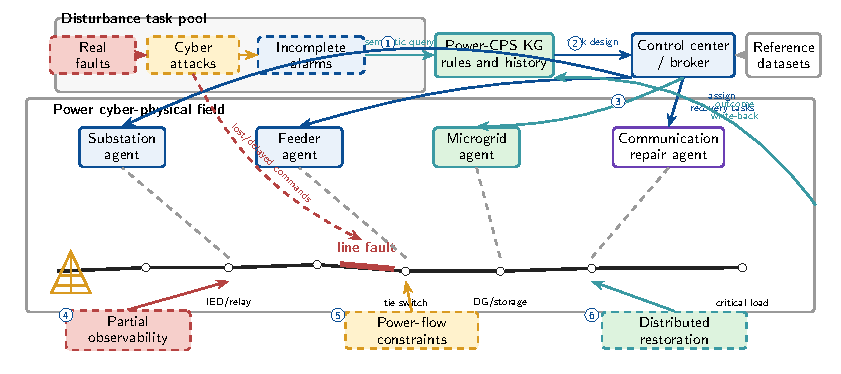
\includegraphics[width=\textwidth]{figures/power_cps_scenario.pdf}
\caption{Illustrative recovery setting in a power cyber-physical system. Physical faults, impaired communication, and incomplete or corrupted observations jointly determine which restoration actions can be trusted and executed.}
\label{fig-scenario}
\end{figure*}

Resilient CPS research has studied cross-layer dependencies among cyber, communication, control, and physical components \cite{zhu2020cross,liao2025surveyresilient}. Existing methods include game-theoretic resilient control, secure or resilient model predictive control, and observer/event-triggered designs for denial-of-service, false-data-injection, and hybrid attacks \cite{game2026hybrid,resilientmpc2025dos,stochastic2025tube,sampled2025observer}. Power-system restoration models have also incorporated communication impairment and cyber-physical operating constraints into reconfiguration and service recovery \cite{zhou2025faultresilient}. In these formulations, runtime inputs usually appear as measurements, estimated states, attack estimates, communication states, or predefined constraints. Recovery studies also make explicit assumptions about diagnosis, attack history, and the recovery module \cite{lu2024recovery}. What remains less explicit is the integrity of a reusable knowledge state assembled from these inputs and later used to authorize recovery actions.

Knowledge graphs (KGs) are useful for representing such dependencies as typed, queryable relations. General KG work covers heterogeneous entities and relations, context, validation, inference, and graph learning \cite{hogan2021knowledgegraphs,reinanda2020knowledge}. CPS studies have used KGs for time-continuous behavior, weighted information dependencies, cross-domain threat modeling, and control reconfiguration \cite{liu2025timecontinuous,wang2025weightedkg,wu2026multidimensional,knowledge2025dynamic}. Incremental causal graphs and KG-assisted verification have also been explored for online attack detection \cite{incremental2026causal,hybridtcdf2026}. These capabilities do not by themselves determine whether the evidence that created a runtime assertion is trustworthy. Three reports can be syntactically distinct yet share one compromised gateway; a valid old report can be replayed after the operating condition has changed. Both cases can alter a graph state without violating its schema.

We call this attack surface \emph{recovery knowledge poisoning}. The path of interest is
\begin{align}
\label{eq-intro-propagation}
&\text{adversarial evidence}\rightarrow\text{recovery knowledge}\nonumber\\
&\qquad\rightarrow\text{action authority}\rightarrow\text{online policy}.
\end{align}
Consider a fabricated controller-availability report. If it is accepted as ordinary recovery knowledge, a remote switching action can pass a semantic prerequisite even though the controller is unavailable. The resulting transition may then enter replay and influence later policy updates after the original report has expired. This is the point at which anomaly detection, a physical safety check, and robust policy optimization solve different problems: none of them alone controls the whole evidence-to-knowledge-to-learning path.

KG-FedMARL addresses that path at three places. Runtime assertions are maintained as temporal beliefs with source identity and provenance. Evidence is calibrated, aged, and grouped by provenance so that one correlated source group has bounded influence. Recovery actions use these beliefs only for evidence-dependent prerequisites; invariant engineering constraints remain the responsibility of an authoritative physical verifier over a conservative state set. A learned surrogate may rank candidates, but it cannot approve field execution.

Online learning uses a separate, slower trust boundary. Each transition is tied to the belief, policy, and verifier versions present at execution. New transitions remain in quarantine until their supporting beliefs, provenance coverage, evidence completeness, and outcomes meet the promotion criteria. Stable and candidate policies are kept separate, and candidate promotion is restricted by a trust-dependent KL radius and shadow evaluation through the same recovery gate. Federated training, heterogeneous action heads, and graph encoders can be used in an implementation, but they have no authority to bypass the local gate or verifier.

We formulate restoration as a constrained decentralized partially observable Markov decision process with four security quantities: belief distortion under bounded evidence compromise, semantic false authorization, correction time after trustworthy evidence resumes, and deviation of the deployed policy. Section~VI derives sufficient bounds for these quantities from the provenance budgets, forgetting factor, calibration error, and policy-promotion constraints. The guarantees are limited to the trust boundary stated in Section~III; they are not a convergence proof for a nonlinear MARL optimizer.

The paper makes three contributions.
\begin{itemize}
\item \emph{Recovery-knowledge threat model.} We define recovery knowledge poisoning for bounded source compromise, fabrication, suppression, replay, delay, and provenance correlation. The model separates protected semantic invariants from runtime assertions inferred from evidence.

\item \emph{Recovery mechanisms with explicit trust boundaries.} KG-FedMARL combines provenance-bounded temporal belief updates, a semantic recovery gate followed by authoritative physical verification, and quarantined online policy adaptation with stable--candidate separation.

\item \emph{Security bounds tied to the recovery pipeline.} We bound belief distortion, semantic false-authorization probability, post-attack correction time, and cumulative deployed-policy drift under the stated assumptions, and evaluate the same quantities in controlled and feeder-level experiments.
\end{itemize}

Section~II reviews related work. Section~III defines the system and threat model. Section~IV gives the restoration formulation and security objectives. Section~V presents KG-FedMARL, Section~VI gives the security analysis, and Section~VII reports the experiments.

\section{RELATED WORK}
This section reviews the literature that determines the design space of KG-FedMARL: cross-layer resilience theory, KG representation for CPSs, cyber-physical restoration, and graph-based MARL. Table~\ref{table-re} summarizes which parts of the full restoration loop are covered by each line of work.

\begin{table*}[t]
	\centering
	\caption{Positioning of KG-FedMARL against representative research lines}
	\label{table-re}
	\setlength{\tabcolsep}{2.2mm}{
	\resizebox{\textwidth}{!}{
		\begin{tabular}{lcccccc}
			\toprule[1.5pt]
			Research line & Cross-layer CPS theory & Dynamic KG semantics & Physical-cyber restoration & MARL decision making & Federated/asynchronous learning & Rule-level safety filter \\
			\midrule
			Cross-layer secure CPS design \cite{zhu2020cross} & $\checkmark$ & $\times$ & $\triangle$ & $\triangle$ & $\times$ & $\triangle$ \\
			KG surveys and KG-ML foundations \cite{hogan2021knowledgegraphs,reinanda2020knowledge,damato2023machine} & $\times$ & $\checkmark$ & $\times$ & $\triangle$ & $\times$ & $\triangle$ \\
			Power/industrial KG modeling \cite{wu2026multidimensional,liu2025timecontinuous,wang2025weightedkg} & $\triangle$ & $\checkmark$ & $\triangle$ & $\times$ & $\times$ & $\triangle$ \\
			Resilient control and coordination \cite{liao2025surveyresilient,game2026hybrid,resilientmpc2025dos} & $\checkmark$ & $\times$ & $\triangle$ & $\triangle$ & $\times$ & $\checkmark$ \\
			Distribution restoration and reconfiguration \cite{zhou2025faultresilient} & $\triangle$ & $\times$ & $\checkmark$ & $\triangle$ & $\times$ & $\checkmark$ \\
			KG-assisted learning/control \cite{rodrigues2026agentic,hybridkgdrl2025,graphzero2025} & $\triangle$ & $\checkmark$ & $\triangle$ & $\checkmark$ & $\triangle$ & $\triangle$ \\
			KG-FedMARL & $\checkmark$ & $\checkmark$ & $\checkmark$ & $\checkmark$ & $\checkmark$ & $\checkmark$ \\
			\bottomrule[1.5pt]
	\end{tabular}}}
	\vspace{1mm}
	\footnotesize{\emph{Note:} $\checkmark$ denotes a core focus, $\triangle$ denotes partial coverage, and $\times$ denotes limited coverage.}
\end{table*}

\subsection{Cross-Layer Resilience in Cyber-Physical Systems}
Cross-layer CPS resilience starts from the observation that an attack or fault can propagate through several layers before its operational effect is visible. The decision- and game-theoretic treatment by Zhu and Xu is the theoretical basis used here: resilience is shaped by incomplete information, strategic interaction, layer coupling, and the timing of defensive responses \cite{zhu2020cross}. Recent control studies instantiate parts of this view through secure MPC, resilient observers, game-theoretic mitigation, event-triggered control, anti-windup fault tolerance, sliding-mode control, and distributed consensus under malicious attacks \cite{game2026hybrid,resilientmpc2025dos,adaptive2025event,antiwindup2025secure,fixedtime2025sliding,fullydistributed2025consensus}. Their strength is mathematical control analysis. Their limitation for the present restoration task is that the cyber-physical relations needed by operators are usually not explicit data objects. KG-FedMARL keeps the cross-layer formulation but exposes those relations as typed graph facts that can be queried by a decision algorithm.

\subsection{Knowledge Graphs and Neuro-Symbolic Learning}
KG research offers three ingredients needed by restoration: typed relations for heterogeneous data, symbolic rules for validation, and embeddings or graph neural networks for learning over relational neighborhoods \cite{hogan2021knowledgegraphs}. Information-retrieval work adds practical concerns such as entity linking, relation explanation, graph completion, and quality estimation \cite{reinanda2020knowledge}. Recent KG-ML studies describe the remaining gap between symbolic semantics and data-driven learning, arguing that future systems should allow each side to improve the other \cite{damato2023machine}. KG-FedMARL uses this neuro-symbolic stance directly: graph facts constrain actions, graph neighborhoods become policy inputs, and executed actions update graph memory.

For CPSs and power infrastructure, KGs have been used to model temporal system behavior, weighted information dependencies, power-grid threats, and dynamic control reconfiguration \cite{liu2025timecontinuous,wang2025weightedkg,wu2026multidimensional,knowledge2025dynamic}. Causal graph learning and KG verification have also been studied for online cyberattack detection in industrial systems \cite{incremental2026causal,hybridtcdf2026}. These studies show that a graph can carry operational semantics, but most stop before action selection. The present work extends this line by connecting KG reasoning to a constrained multi-agent restoration policy.

\subsection{Resilient Restoration of Power CPSs}
Power distribution restoration has long studied fault isolation, switch reconfiguration, load recovery, distributed-generation support, and radiality or power-flow constraints. More recent cyber-physical restoration work adds communication recovery and situational-awareness constraints. Hybrid flow constraints and minimum-cost communication restoration, for example, can coordinate feeder self-healing with impaired communication \cite{zhou2025faultresilient}. Resilient coordination surveys similarly emphasize that malicious CPS events exploit topology, information channels, and physical dynamics at the same time \cite{liao2025surveyresilient}. The remaining issue is representation. Static coupling matrices are hard to update when an outage evolves; handcrafted constraints are hard to reuse across scenarios. KG-FedMARL models those couplings as dynamic typed relations and uses the affected subgraph as the unit of restoration reasoning.

\subsection{Multi-Agent Reinforcement Learning and Graph-Based Decision}
MARL is a natural tool when several controllers act locally but influence a shared objective. Graph neural networks are useful in power systems because the relevant dependencies are non-Euclidean and topology dependent \cite{gnnpowersystems2024}. Graph reinforcement learning has been studied for scalable zero-day behavioral intrusion detection, and hybrid KG-deep RL has been explored for EV-charging anomaly detection \cite{graphzero2025,hybridkgdrl2025}. Agentic-control frameworks have also begun to combine KG retrieval with game-theoretic multi-agent learning \cite{rodrigues2026agentic}. KG-FedMARL differs in its execution boundary: it targets restoration actions in a power CPS, checks candidate actions before field execution, and trains through a federated asynchronous protocol that reflects distributed operational ownership.

\begin{table}[t]
	\centering
	\caption{Key notations}
	\label{table-notations1}
	\setlength{\tabcolsep}{1.2mm}{
	\begin{tabular}{ll}
		\toprule[1.5pt]
		Notation & Definition \\
		\midrule
		$\mathcal{G}^{p}$ & Physical power network graph \\
		$\mathcal{G}^{c}$ & Cyber communication and control graph \\
		$\mathcal{K}_t$ & Dynamic power-CPS knowledge graph at time $t$ \\
		$\mathcal{E},\mathcal{R},\mathcal{X}$ & Entity, relation, and attribute sets in $\mathcal{K}_t$ \\
		$\mathcal{F}_t$ & Fault and attack evidence observed at time $t$ \\
		$\mathcal{Z}_t$ & Aligned evidence-event set at time $t$ \\
		$\mathcal{O}_t$ & Graph-operation set applied to $\mathcal{K}_t$ \\
		$\mathcal{G}^{task}_t$ & Fault-affected task subgraph extracted from $\mathcal{K}_t$ \\
		$s_t$ & Global semantic state vector encoded from $\mathcal{G}^{task}_t$ \\
		$o_t^i$ & Local observation of restoration agent $i$ \\
		$a_t^i$ & Local restoration action of agent $i$ \\
		$\mathbf{a}_t$ & Joint restoration action \\
		$\mathcal{A}^{safe}(s_t)$ & Rule- and physics-feasible joint action set \\
		$\eta_t$ & Recovered load ratio after action execution \\
		$N_{\rm viol}(t)$ & Number or severity of safety violations \\
		$\psi,\theta_g,\nu_i,\phi$ & Shared encoder, role head, local adapter, and critic parameters \\
		$\omega_i$ & Federated aggregation weight of client $i$ \\
		\bottomrule[1.5pt]
	\end{tabular}}
\end{table}

\section{SYSTEM MODEL}
This section defines the cross-layer power-CPS model and the dynamic knowledge graph used by KG-FedMARL. Table~\ref{table-notations1} lists the main notation.

\subsection{Cross-Layer Power-CPS Architecture}
We model a power CPS as an interdependent system
\begin{align}
\label{eq-cross-layer-system}
\mathcal{S}=\{\mathcal{G}^{p},\mathcal{G}^{c},\mathcal{D},\mathcal{U},\mathcal{C}\},
\end{align}
where $\mathcal{G}^{p}=(\mathcal{V}^{p},\mathcal{L}^{p})$ is the physical power network, $\mathcal{G}^{c}=(\mathcal{V}^{c},\mathcal{L}^{c})$ is the cyber communication and control network, $\mathcal{D}$ denotes distributed measurement and actuation devices, $\mathcal{U}$ denotes controllable restoration resources, and $\mathcal{C}$ denotes operational constraints.

The physical node set $\mathcal{V}^{p}$ contains buses, feeders, transformers, generators, energy-storage units, loads, distributed generators, and microgrid interfaces. Physical lines $\mathcal{L}^{p}$ carry power flows and are constrained by radiality, voltage magnitude, current limits, switch states, protection coordination, and resource capacities. The cyber node set $\mathcal{V}^{c}$ contains control centers, substation controllers, intelligent electronic devices, communication relays, edge servers, and monitoring terminals. Cyber links $\mathcal{L}^{c}$ transmit measurements, commands, protection messages, model updates, and restoration coordination signals.

Physical and cyber layers are coupled by typed dependencies. A cyber controller may supervise a physical breaker; a sensor may measure a bus voltage; a communication path may be required before a remote switch command can be executed; a power-line fault may also damage fiber links installed on the same corridor. We represent these dependencies as a cross-layer relation set
\begin{align}
\label{eq-coupling-relation}
\mathcal{R}^{pc}=\{(u,r,v)\mid u\in\mathcal{V}^{p}\cup\mathcal{V}^{c}, v\in\mathcal{V}^{p}\cup\mathcal{V}^{c}\}.
\end{align}
This explicit relation set follows the cross-layer CPS design principle that resilience emerges from inter-layer coordination rather than isolated layer hardening \cite{zhu2020cross}.

\subsection{Cross-Layer Dependency Classes}
For restoration, not every dependency has the same decision meaning. We divide $\mathcal{R}^{pc}$ into four classes that are checked at different points in the KG-FedMARL loop.

\emph{Observation dependencies} connect a physical quantity to the sensing, communication, and trust chain that makes it observable. A voltage value at bus $v$ is usable only if the associated sensor, communication route, timestamp, and trust attribute are acceptable. \emph{Actuation dependencies} connect an action to the cyber path, authorization rule, and device state required for execution. \emph{Constraint dependencies} connect actions and devices to radiality, voltage, thermal, protection, load-priority, and communication-availability constraints. \emph{Damage dependencies} represent co-location or causal relations through which a physical event can degrade cyber resources, or a cyber attack can corrupt physical-state estimation.

This separation matters because the restoration controller should not treat all missing information as the same kind of uncertainty. A missing measurement affects state estimation; an unavailable command path affects action feasibility; an active protection rule affects admissibility; and a suspected data attack affects trust. KG-FedMARL keeps these distinctions in the KG relation vocabulary so that the policy input and the safety filter receive different evidence for different failure mechanisms.

\subsection{Fault, Attack, and Restoration Process}
At each decision time $t$, the system receives incomplete evidence $\mathcal{F}_t$ from protection devices, supervisory control and data acquisition logs, phasor measurements, alarms, and communication status. The evidence may include line trips, abnormal voltage, unavailable sensors, delayed commands, corrupted measurements, and suspected cyber attacks. The true system condition is partially observed because faults can disable the sensing and communication channels needed to diagnose them.

Restoration actions include switch opening/closing, feeder reconfiguration, load transfer, distributed-generator dispatch, energy-storage support, microgrid islanding or reconnection, communication-path repair, relay/protection-rule adjustment, and temporary load shedding. Not every action is feasible in every state. An action must satisfy both physical constraints and cyber prerequisites. For example, closing a tie switch is invalid if it creates a loop in a radial feeder, overloads a line, violates a voltage bound, or relies on an unavailable control path.

We describe the system transition as
\begin{align}
\label{eq-system-transition}
x_{t+1}=f(x_t,\mathbf{a}_t,\xi_t),
\end{align}
where $x_t$ is the latent cross-layer state, $\mathbf{a}_t$ is the joint restoration action, and $\xi_t$ captures stochastic fault evolution, demand fluctuation, renewable output, cyber delay, and model uncertainty. The learning agents cannot observe $x_t$ directly; instead they use local observations and graph-derived semantic states.

\subsection{Dynamic Power-CPS Knowledge Graph}
The dynamic knowledge graph at time $t$ is
\begin{align}
\label{eq-kg}
\mathcal{K}_t=(\mathcal{E}_t,\mathcal{R}_t,\mathcal{X}_t,\mathcal{T}_t),
\end{align}
where $\mathcal{E}_t$ is the entity set, $\mathcal{R}_t$ is the relation set, $\mathcal{X}_t$ stores attributes, and $\mathcal{T}_t$ stores temporal validity and provenance. The graph follows the general KG view of typed entities, relations, ontologies, rules, reasoning, and embeddings \cite{hogan2021knowledgegraphs,reinanda2020knowledge}. In KG-FedMARL, the entity set includes four restoration-oriented classes:
\begin{itemize}
	\item \emph{Device entities}: buses, lines, breakers, transformers, sensors, relays, controllers, communication nodes, generators, loads, storage units, and microgrids.
	\item \emph{State entities}: energized/de-energized state, load level, voltage, frequency, communication availability, fault probability, device health, and cyber trust.
	\item \emph{Action entities}: switching, load transfer, generator dispatch, storage charging/discharging, microgrid islanding, communication rerouting, and emergency shedding.
	\item \emph{Rule entities}: protection settings, radiality rules, voltage/current limits, control authorization, operation manuals, safety constraints, and restoration priorities.
\end{itemize}

The relation vocabulary is designed for restoration rather than generic asset management. It includes \emph{topologically-connected}, \emph{communicates-with}, \emph{measures}, \emph{controls}, \emph{depends-on}, \emph{causes}, \emph{relieves}, \emph{violates}, \emph{satisfies}, \emph{precedes}, and \emph{similar-to}. A typed triple $(e_h,r,e_t)$ can therefore state that a relay controls a breaker, a breaker connects two buses, a communication route is needed by a switch action, or a previous load-transfer action relieved a similar fault.

The graph is updated online rather than rebuilt from scratch. Raw evidence $\mathcal{F}_t$ is first aligned to an evidence-event set
\begin{align}
\label{eq-evidence-event}
\mathcal{Z}_t=\{z=(e_s,\kappa,e_o,v_z,t,c_z,p_z)\},
\end{align}
where $e_s$ is the source entity, $\kappa$ is the evidence type, $e_o$ is the affected entity or relation, $v_z$ is the reported value, $c_z\in[0,1]$ is evidence confidence, and $p_z$ stores provenance. Each event is converted by a rule-and-scoring mapper $\mathcal{M}_{\psi}$ into graph operations
\begin{align}
\label{eq-graph-ops}
\mathcal{O}_t&=\mathcal{M}_{\psi}(\mathcal{Z}_t,\mathcal{K}_t) \nonumber\\
&=\{\textsc{AddE},\textsc{AddR},\textsc{UpdateX},\textsc{DeactivateR}\}.
\end{align}
The resulting graph update is
\begin{align}
\label{eq-kg-update}
\mathcal{K}_{t+1}=\textsc{Apply}\left(\mathcal{K}_t,\mathcal{O}_t,\mathbf{p}_t\right),
\end{align}
where every changed fact receives a timestamp, validity interval, source tag, and confidence. Uncertain cyber or measurement evidence does not physically remove a relation. It adds a state entity and reduces a confidence or trust attribute. A relation is deactivated only when the evidence is confirmed, and even then the old relation is retained with an expired validity interval for audit and replay.

\begin{table*}[t]
	\centering
	\caption{Evidence-to-knowledge-graph update rules used by KG-FedMARL}
	\label{table-evidence-update}
	\setlength{\tabcolsep}{2.0mm}{
	\resizebox{\textwidth}{!}{
	\begin{tabular}{llll}
		\toprule[1.5pt]
		Evidence event & Entity operation & Relation operation & Attribute operation \\
		\midrule
		Line trip or breaker alarm & Add \texttt{FaultState} for the line, breaker, or feeder & Add \texttt{affects} links to buses, loads, sensors, and candidate actions & Set line status, fault probability, isolation time, and evidence confidence \\
		Measurement anomaly & Add \texttt{MeasurementAnomaly} or \texttt{SuspectedAttackState} with timestamp & Add \texttt{suspected-corrupts}; keep \texttt{measures} but lower its confidence & Decrease measurement-path trust and increase observation uncertainty \\
		Controller unavailable or delayed command & Add \texttt{UnavailableControllerState} or \texttt{DelayState} & Temporarily deactivate \texttt{can-execute} or \texttt{requires-route} if confirmed & Update reachability, latency, authorization, and command-success probability \\
		Communication reroute or repair & Add \texttt{RepairState} for the affected route & Add or reactivate \texttt{communicates-with} and \texttt{supports-command} & Update bandwidth, latency, route reliability, and repair time \\
		Executed restoration action & Add \texttt{RestorationOutcome} linked to the action and context & Add \texttt{relieves}, \texttt{violates}, or \texttt{similar-to} explanation paths & Update load recovery, violation count, cyber cost, and action success memory \\
		\bottomrule[1.5pt]
	\end{tabular}}}
\end{table*}

For soft evidence, confidence is updated by a bounded exponential rule
\begin{align}
\label{eq-confidence-update}
c_{q,t+1}=(1-\alpha)c_{q,t}+\alpha\,\varsigma(z,q),
\end{align}
where $c_{q,t}$ is the confidence of a fact, relation, or attribute $q$ and $\varsigma(z,q)$ is the evidence-specific support score returned by $\mathcal{M}_{\psi}$. For action entities, the graph maintains a reliability attribute
\begin{align}
\label{eq-action-reliability}
\begin{split}
p_{succ}(a,r_c)\leftarrow &(1-\beta)p_{succ}(a,r_c)\\
&+\beta\mathbb{I}\{\mathbf{y}_t\ \text{passes acceptance tests}\},
\end{split}
\end{align}
where $r_c$ denotes the relevant restoration context, such as a fault type, measurement-trust pattern, controller availability state, and cyber-route condition. This update turns the KG into an experience memory: a future task subgraph can retrieve which action paths previously restored load without violating constraints under a similar context.

\subsection{Task Subgraph and Semantic State}
Given current evidence $\mathcal{F}_t$, KG-FedMARL extracts a $k$-hop task subgraph
\begin{align}
\label{eq-task-subgraph}
\mathcal{G}^{task}_t=(\mathcal{V}^{task}_t,\mathcal{E}^{task}_t)
\end{align}
around the affected devices, unavailable cyber nodes, candidate restoration actions, and active constraints. Each node $v\in\mathcal{V}^{task}_t$ has a feature vector
\begin{align}
\label{eq-node-feature}
\mathbf{x}_v=[\mathbf{e}^{type}_v,\mathbf{z}^{op}_v,p^{fault}_v,p^{succ}_v,\mathbf{z}^{time}_v],
\end{align}
where $\mathbf{e}^{type}_v$ encodes entity type, $\mathbf{z}^{op}_v$ stores normalized operating attributes, $p^{fault}_v$ is fault probability, $p^{succ}_v$ is historical action success rate when applicable, and $\mathbf{z}^{time}_v$ encodes temporal recency and duration.

A relation-aware graph-attention encoder maps the task subgraph into a global semantic vector. For relation $r_{uv}$ between nodes $u$ and $v$, the attention logit is
\begin{align}
\label{eq-rel-attention}
e_{uv}^{\ell}=\text{LeakyReLU}\left(\mathbf{q}^{\ell\top}
\left[\mathbf{W}^{\ell}\mathbf{h}_{u}^{\ell};\mathbf{W}^{\ell}\mathbf{h}_{v}^{\ell};\mathbf{W}_{r}^{\ell}\mathbf{r}_{uv}\right]\right),
\end{align}
and
\begin{align}
\label{eq-attention-normalize}
\alpha_{uv}^{\ell}=\frac{\exp(e_{uv}^{\ell})}{\sum_{w\in\mathcal{N}(v)}\exp(e_{wv}^{\ell})}.
\end{align}
The node update is
\begin{align}
\label{eq-gat}
\mathbf{h}_{v}^{\ell+1}=\sigma\left(\sum_{u\in\mathcal{N}(v)}\alpha_{uv}^{\ell}\mathbf{W}^{\ell}\mathbf{h}_{u}^{\ell}\right),
\end{align}
where $\mathbf{r}_{uv}$ encodes the relation type and confidence. A pooling operator then produces
\begin{align}
\label{eq-semantic-state}
s_t=\text{POOL}\left(\{\mathbf{h}_{v}^{L}:v\in\mathcal{V}^{task}_t\}\right).
\end{align}
Each agent $i$ receives the augmented observation
\begin{align}
\label{eq-agent-state}
\tilde{s}_t^i=[o_t^i;s_t],
\end{align}
which combines local device or feeder information with global cross-layer semantics.

\section{PROBLEM FORMULATION}
\label{sec-problem-formulation}
This section formalizes resilient restoration under adversarial recovery knowledge. The formulation separates four issues that were conflated in the original manuscript: partial observability, evidence-dependent action admissibility, worst-case recovery performance, and the security objective of bounding the propagation of erroneous knowledge. The attacker is modeled through the observation and evidence processes defined in Section~\ref{sec-system-model}, rather than as a cooperative decision agent.

\subsection{Constrained Dec-POMDP under Adversarial Knowledge}
\label{subsec-decpomdp}
Let $\mathcal{I}=\{1,\ldots,N\}$ denote the set of restoration agents. Because each agent observes only a local part of the PCPS and the recovery knowledge state summarizes time-dependent evidence history, we model restoration as a constrained decentralized partially observable Markov decision process (C-Dec-POMDP)
\begin{align}
\label{eq-cdecpomdp}
\mathcal{M}_{\rm rec}=\left\langle
\mathcal{I},\mathcal{X},\{\mathbb{U}_i\}_{i\in\mathcal{I}},
P,\{\mathcal{O}_i\}_{i\in\mathcal{I}},O,R,\mathcal{C},\gamma
\right\rangle,
\end{align}
where $\mathcal{X}$ is the latent cross-layer state space, $\mathbb{U}_i$ is the action space of agent $i$, $P(x_{t+1}\mid x_t,\mathbf{a}_t)$ is the state-transition kernel, $\mathcal{O}_i$ is the local observation space, $O$ is the observation model, $R$ is the cooperative restoration reward, $\mathcal{C}$ is the constraint set, and $\gamma\in(0,1)$ is the discount factor. We use $\mathbb{U}_i$ for action spaces to avoid overloading $\mathcal{A}_t$, which denotes dynamic KG assertions in Section~\ref{subsec-recovery-knowledge-plane}.

At time $t$, agent $i$ receives a local observation $o_{i,t}$ and has access to the task-relevant portion of the recovery belief state $\mathcal{B}_t$. Its decision information is written abstractly as
\begin{align}
\label{eq-information-state}
\iota_{i,t}=\big(\tau_{i,t},\mathcal{B}^{i}_t\big),
\end{align}
where $\tau_{i,t}=(o_{i,0},a_{i,0},\ldots,o_{i,t})$ is the local action--observation history and $\mathcal{B}^{i}_t\subseteq\mathcal{B}_t$ contains the recovery beliefs relevant to the agent's current task. The concrete extraction and encoding of $\mathcal{B}^{i}_t$ are implementation choices deferred to Section~V. A decentralized policy selects
\begin{align}
\label{eq-decentralized-policy}
a_{i,t}\sim\pi_i(\cdot\mid\iota_{i,t}),
\end{align}
and the joint candidate action is $\mathbf{a}_t=(a_{1,t},\ldots,a_{N,t})$.

The adversary affects decision making indirectly by manipulating admissible evidence streams within the budget $\mathcal{B}_{A}$ in Eq.~\ref{eq-attack-budget}. Thus the observation and knowledge processes are attack dependent, whereas the physical transition kernel remains governed by the PCPS dynamics in Eq.~\ref{eq-system-transition}. This distinction is important: the security problem is not merely to tolerate exogenous state disturbances, but to prevent corrupted observations from becoming trusted recovery knowledge and then executable control authority.

\subsection{Risk-Aware Action Admissibility}
\label{subsec-risk-admissibility}
We partition the restoration constraints into invariant engineering constraints and evidence-dependent prerequisites,
\begin{align}
\label{eq-constraint-partition}
\mathcal{C}=\mathcal{C}^{\rm inv}\cup\mathcal{C}^{\rm evid}_t.
\end{align}
The set $\mathcal{C}^{\rm inv}$ contains requirements whose validity does not depend on online attack diagnosis, such as voltage and thermal limits, device ratings, power-balance relations, protection interlocks, and radiality. By contrast, $\mathcal{C}^{\rm evid}_t$ contains runtime conditions inferred from evidence, such as whether a controller is available, whether a command route is reachable, or whether a measurement chain is sufficiently trustworthy for a specific operation.

For a candidate joint action $\mathbf{a}$, let
\begin{align}
\mathcal{Q}(\mathbf{a})=\{q_1,\ldots,q_m\}
\end{align}
be the dynamic assertions that must hold for its cyber-physical execution. Instead of converting each KG assertion into a binary rule, we assign a risk budget $\delta_q\in(0,1)$ and require
\begin{align}
\label{eq-belief-prerequisite}
b_t(q)\ge 1-\delta_q,
\qquad \forall q\in\mathcal{Q}(\mathbf{a}).
\end{align}
The corresponding belief-admissible set is
\begin{align}
\label{eq-belief-admissible-set}
\mathbb{U}^{B}_t=
\left\{\mathbf{a}\ \middle|\
 b_t(q)\ge1-\delta_q,
\ \forall q\in\mathcal{Q}(\mathbf{a})
\right\}.
\end{align}
Equation~\ref{eq-belief-admissible-set} makes uncertainty explicit: insufficient evidence cannot be interpreted as permission. The aggregate semantic risk budget for action $\mathbf{a}$ is constrained by
\begin{align}
\label{eq-semantic-risk-budget}
\sum_{q\in\mathcal{Q}(\mathbf{a})}\delta_q\le\bar{\delta}_{B},
\end{align}
where $\bar{\delta}_{B}$ is selected according to the criticality of the restoration operation.

Invariant safety is checked independently of the belief gate. Let $\widehat{\mathcal{X}}_t$ be a conservative set of physical states consistent with the currently trusted measurements and uncertainty bounds. We define
\begin{align}
\label{eq-invariant-admissible-set}
\mathbb{U}^{\rm inv}_t=
\Big\{\mathbf{a}\ \Big|\
&g_k(x,\mathbf{a})\le0,\ \forall k,\\
&h_l(x,\mathbf{a})=0,\ \forall l,
\ \forall x\in\widehat{\mathcal{X}}_t
\Big\},\nonumber
\end{align}
where $g_k$ and $h_l$ represent inequality and equality/structural constraints, respectively. The final admissible action set is
\begin{align}
\label{eq-final-admissible-set}
\mathbb{U}^{\rm adm}_t
=\mathbb{U}^{B}_t\cap\mathbb{U}^{\rm inv}_t.
\end{align}
A learned surrogate may later reduce the number of candidates sent to exact verification, but it cannot enlarge $\mathbb{U}^{\rm inv}_t$ and therefore has no independent authorization authority. If no nontrivial action is admissible, the controller executes a certified fallback action $\mathbf{a}^{\rm fb}_t\in\mathbb{U}^{\rm inv}_t$, such as maintaining isolation, retaining local control, or shedding a bounded amount of load.

\subsection{Robust Recovery Objective}
\label{subsec-robust-objective}
Let $\mathcal{L}$ be the set of loads, $P_l$ the nominal demand of load $l$, $w_l>0$ its service priority, and $y_{l,t}\in[0,1]$ its restored fraction at time $t$. The weighted restored-service ratio is
\begin{align}
\label{eq-weighted-recovery-ratio}
\eta_t=
\frac{\sum_{l\in\mathcal{L}}w_lP_l y_{l,t}}
{\sum_{l\in\mathcal{L}}w_lP_l}.
\end{align}
We use safety as a hard constraint rather than allowing a large restoration reward to compensate for an unsafe operation. The stage reward therefore captures service recovery and operational costs,
\begin{align}
\label{eq-robust-reward}
R_t=
\lambda_{\eta}\eta_t
-\lambda_{s}C^{\rm shed}_t
-\lambda_{o}C^{\rm op}_t
-\lambda_{c}C^{\rm cyber}_t
-\lambda_{f}C^{\rm fb}_t,
\end{align}
where $C^{\rm shed}_t$, $C^{\rm op}_t$, $C^{\rm cyber}_t$, and $C^{\rm fb}_t$ denote critical-load curtailment, switching/dispatch cost, cyber-resource recovery cost, and fallback-service loss, respectively.

Let $\mathfrak{A}(\mathcal{B}_{A})$ denote the set of adversaries satisfying the capability and budget assumptions in Section~\ref{subsec-threat-model}. We seek a recovery policy and online belief-update rule that maximize worst-case expected recovery performance,
\begin{align}
\label{eq-minimax-objective}
\max_{\Pi,F_B}\ \inf_{\mathscr{A}\in\mathfrak{A}(\mathcal{B}_{A})}
\mathbb{E}_{\mathscr{A}}
\left[\sum_{t=0}^{T}\gamma^t R_t\right],
\end{align}
where $\Pi=\{\pi_i\}_{i\in\mathcal{I}}$ and
$F_B$ denotes the online update mapping that produces $\mathcal{B}_{t+1}$ from the previous belief state and newly received evidence. The optimization in Eq.~\ref{eq-minimax-objective} is subject to
\begin{align}
\label{eq-execution-constraint}
\mathbf{a}^{\rm exec}_t\in\mathbb{U}^{\rm adm}_t,
\end{align}
and to the physical safety and recovery requirements
\begin{align}
\label{eq-safety-probability}
\Pr\left(x_t\in\mathcal{X}_{\rm unsafe}\right)&\le\delta_x,
\qquad 0\le t\le T,\\
\label{eq-recovery-liveness}
\Pr\left(\exists t\le T_{\max}:x_t\in\mathcal{X}_{\rm tar}\right)&\ge1-\delta_r.
\end{align}
Here $\mathcal{X}_{\rm unsafe}$ and $\mathcal{X}_{\rm tar}$ denote the unsafe and target recovery sets, respectively. Equation~\ref{eq-recovery-liveness} prevents an overly conservative knowledge gate from achieving safety simply by refusing all useful restoration actions.

\subsection{Security Objectives: Bounding Knowledge Propagation}
\label{subsec-security-objectives}
The distinguishing security objective of this work is to bound how far adversarial evidence can propagate through the recovery loop. We formalize this requirement at the knowledge, action, correction, and policy levels. These properties are design targets in this section; Section~V provides the mechanisms and the later theoretical analysis establishes sufficient conditions for them.

\emph{1) Bounded belief distortion.}
Let $\mathcal{B}^{0}_t$ denote the counterfactual recovery belief state generated from uncompromised evidence under the same physical trajectory, and let $\mathcal{B}^{A}_t$ denote the belief state under an admissible attack. For the task-relevant assertion set $\mathcal{Q}_t$, define
\begin{align}
\label{eq-belief-distance}
D_B(\mathcal{B}^{A}_t,\mathcal{B}^{0}_t)
=\sum_{q\in\mathcal{Q}_t}\omega_q
\left|b^{A}_t(q)-b^{0}_t(q)\right|,
\qquad \sum_q\omega_q=1.
\end{align}
The first objective is the existence of a finite attack-budget-dependent bound
\begin{align}
\label{eq-bounded-belief-distortion}
\sup_{t\le T}
D_B(\mathcal{B}^{A}_t,\mathcal{B}^{0}_t)
\le \varepsilon_B(\mathcal{B}_{A}).
\end{align}
This rules out unbounded accumulation of influence from a bounded number of compromised provenance groups.

\emph{2) Bounded false authorization.}
Let $\mathbb{U}^{\star}_t$ denote the action set that would be semantically admissible if the ground-truth values $q_t^{\star}$ of all prerequisites were known. A false authorization occurs when an action is admitted by the online belief state but is not contained in $\mathbb{U}^{\star}_t$. We require
\begin{align}
\label{eq-false-authorization-bound}
\Pr\left(
\mathbf{a}^{\rm exec}_t\in
\mathbb{U}^{\rm adm}_t\setminus\mathbb{U}^{\star}_t
\right)
\le \delta_{\rm auth}.
\end{align}
This objective formalizes the desired barrier between erroneous knowledge and field control authority.

\emph{3) Finite correction after poisoning.}
Suppose an attack affecting assertion $q$ ceases at time $t_a$ and sufficient uncompromised evidence resumes. For tolerance $\epsilon_{\rm corr}>0$, define the correction time
\begin{align}
\label{eq-correction-time}
T_{\rm corr}(q)=
\inf\left\{k\ge0:\left|b^{A}_{t_a+k}(q)-b^{0}_{t_a+k}(q)\right|\le\epsilon_{\rm corr}\right\}.
\end{align}
We seek conditions under which
\begin{align}
\label{eq-finite-correction}
T_{\rm corr}(q)\le\overline{T}_{\rm corr}
\end{align}
for all task-critical assertions whose honest evidence becomes observable again. This prevents stale or poisoned recovery facts from persisting indefinitely after the attack ends.

\emph{4) Bounded knowledge-to-policy propagation.}
Let $\Pi^{A}_t$ and $\Pi^{0}_t$ denote online policies adapted from attacked and uncompromised recovery knowledge, respectively. We measure adversarially induced policy deviation by
\begin{align}
\label{eq-policy-distance}
D_{\pi}(\Pi^{A}_t,\Pi^{0}_t)
=\frac{1}{N}\sum_{i=1}^{N}
\mathbb{E}_{\iota\sim\mu_t}
\left[
D_{\rm KL}
\left(
\pi^{A}_i(\cdot\mid\iota)
\,\|\,
\pi^{0}_i(\cdot\mid\iota)
\right)
\right],
\end{align}
where $\mu_t$ is the task-relevant information-state distribution. The required propagation bound is
\begin{align}
\label{eq-policy-propagation-bound}
D_{\pi}(\Pi^{A}_t,\Pi^{0}_t)
\le\varepsilon_{\pi}(\mathcal{B}_{A}).
\end{align}
The mechanism in Section~V enforces this objective by separating fast knowledge updates from slower trust-gated policy adaptation, so that a newly inserted or uncertain KG assertion cannot immediately alter the deployed recovery policy.

Together, Eqs.~\ref{eq-bounded-belief-distortion}--\ref{eq-policy-propagation-bound} define the core security problem addressed by this paper: under incomplete, stale, conflicting, and partially adversarial recovery evidence, maintain an online knowledge state whose error remains bounded, prevent that error from directly authorizing unsafe recovery actions, correct poisoned knowledge within finite time once trustworthy evidence returns, and limit the resulting deviation of online recovery policies.
\section{PROVENANCE-AWARE TEMPORAL BELIEF GRAPH}
\label{sec-patbg}
Sections~\ref{sec-patbg}--\ref{sec-trust-policy} constitute the redesigned KG-FedMARL framework. This section addresses the first security objective in Section~\ref{subsec-security-objectives}: a bounded and recoverable online knowledge state under incomplete, stale, conflicting, and partially adversarial evidence. The key design is to treat provenance, temporal validity, and source reliability as part of belief formation rather than as passive metadata.

\subsection{Evidence Reliability and Provenance Dependence}
For an evidence event $z_j=(q_j,v_j,s_j,t_j^e,t_j^r,c_j^{src},p_j)$ defined in Eq.~\ref{eq-evidence-event}, we first calibrate the source-reported confidence by a source-specific mapping $\mathsf{Cal}_{s_j}(\cdot)$ and compute
\begin{align}
\label{eq-evidence-raw-weight}
\bar w_j(t)=\hat c_j\,\rho_{s_j}(t)\,\phi_{age}(z_j,t)\,\phi_{con}(z_j,t),
\end{align}
where $\hat c_j=\mathsf{Cal}_{s_j}(c_j^{src})$, $\rho_{s_j}(t)\in[0,1]$ is the historical reliability of source $s_j$, $\phi_{age}\in[0,1]$ discounts stale evidence, and $\phi_{con}\in[0,1]$ measures consistency with trusted invariants and currently corroborated evidence. We use
\begin{align}
\label{eq-age-decay}
\phi_{age}(z_j,t)=\exp\left[-\lambda_a\max(0,t-t_j^e)\right]
\end{align}
when the event time is credible; otherwise the receive time $t_j^r$ is used. The consistency factor is implementation dependent but must be computed only from trusted invariants or corroborated evidence; it must not reuse the same unverified report as both evidence and verifier.

Multiple reports can share a compromised upstream component. Let $g(z_j)$ denote the independent provenance group of evidence $z_j$ obtained from $\mathcal{P}_t$. For group $g$, define the uncapped absolute contribution
\begin{align}
U_g(t)=\sum_{j:g(z_j)=g}\bar w_j(t)\,|\ell_j(q_j)|,
\end{align}
where $\ell_j(q)$ is a signed evidence log-likelihood ratio. The provenance cap is
\begin{align}
\label{eq-provenance-cap}
\kappa_g(t)=\min\left(1,\frac{\beta_g}{U_g(t)+\epsilon}\right),
\end{align}
and the effective evidence contribution is
\begin{align}
\label{eq-effective-evidence}
u_j(t)=\operatorname{clip}\!\left(\kappa_{g(z_j)}(t)\bar w_j(t)\ell_j(q_j),-\beta_z,\beta_z\right).
\end{align}
Hence, duplicating reports behind the same provenance root cannot increase the total influence of that root beyond $\beta_g$, while $\beta_z$ further bounds the contribution of a single event.

\subsection{Bounded Temporal Belief Update}
For each dynamic assertion $q$, let
\begin{align}
L_t(q)=\log\frac{b_t(q)}{1-b_t(q)},\qquad
L_0(q)=\log\frac{b_0(q)}{1-b_0(q)}
\end{align}
denote its current and prior log-odds. The update rule is
\begin{align}
\label{eq-bounded-belief-update}
L_{t+1}(q)=L_0(q)+\lambda_f\big(L_t(q)-L_0(q)\big)
+\sum_{z_j\in\mathcal{Z}_t(q)}u_j(t),
\end{align}
where $\lambda_f\in(0,1)$ controls temporal retention and $\mathcal{Z}_t(q)$ is the evidence addressing $q$ during the current window. The posterior belief is
\begin{align}
\label{eq-belief-sigmoid}
b_{t+1}(q)=\sigma\big(L_{t+1}(q)\big).
\end{align}
Equation~\ref{eq-bounded-belief-update} has two security effects. First, provenance and per-event clipping make the one-step adversarial influence finite. Second, in the absence of continued support, historical evidence decays toward the prior instead of persisting indefinitely.

Source reliability is updated only when an event becomes verifiable through authenticated repair records, redundant trusted measurements, or post-action physical outcomes. For source $s$, we maintain discounted Beta parameters
\begin{align}
\alpha_s^{t+1}&=\lambda_\rho\alpha_s^t+n_s^{+}(t),\\
\beta_s^{t+1}&=\lambda_\rho\beta_s^t+n_s^{-}(t),
\end{align}
and set
\begin{align}
\label{eq-source-reliability}
\rho_s(t+1)=\frac{\alpha_s^{t+1}}{\alpha_s^{t+1}+\beta_s^{t+1}},
\end{align}
where $n_s^{+}$ and $n_s^{-}$ are counts of newly verified consistent and inconsistent reports. Unverified observations do not directly increase source trust.

The task-relevant knowledge state is extracted after belief update rather than before it. A query returns assertions, prerequisites, temporal validity, and provenance summaries needed by the current disturbance. Graph neural encoding may be used to compress this subgraph for policy input, but the security semantics remain in $b_t(q)$, provenance groups, and validity intervals; they are not replaced by an uninterpretable embedding.

\begin{algorithm}[t]
\caption{Provenance-Aware Temporal Belief Update}
\label{alg-patb}
\KwIn{Current belief graph $\mathcal{G}_t^B$; evidence batch $\mathcal{Z}_t$; verified feedback $\mathcal{Y}_t$; parameters $\lambda_a,\lambda_f,\lambda_\rho,\beta_z,\{\beta_g\}$}
\KwOut{Updated belief graph $\mathcal{G}_{t+1}^B$}
Update source posteriors $(\alpha_s,\beta_s)$ only from verified feedback $\mathcal{Y}_t$ and compute $\rho_s$ by Eq.~\ref{eq-source-reliability}\;
Authenticate source identities, record receive times, and discard malformed or unverifiable messages\;
Group valid evidence by affected assertion $q$ and independent provenance root $g$\;
\ForEach{evidence $z_j$}{
  Calibrate $c_j^{src}$ to $\hat c_j$ and compute $\phi_{age}(z_j,t)$ and $\phi_{con}(z_j,t)$\;
  Compute raw weight $\bar w_j(t)$ using Eq.~\ref{eq-evidence-raw-weight}\;
  Compute signed support $\ell_j(q_j)$\;
}
\ForEach{provenance group $g$}{
  Compute $U_g(t)$ and cap factor $\kappa_g(t)$ using Eq.~\ref{eq-provenance-cap}\;
}
\ForEach{affected assertion $q$}{
  Accumulate clipped group-capped contributions $u_j(t)$\;
  Update $L_{t+1}(q)$ by Eq.~\ref{eq-bounded-belief-update}\;
  Set $b_{t+1}(q)=\sigma(L_{t+1}(q))$ and refresh its validity interval\;
}
Decay untouched dynamic assertions toward their priors according to $\lambda_f$\;
Retain superseded assertion versions and provenance for audit and rollback\;
\Return{$\mathcal{G}_{t+1}^B$}\;
\end{algorithm}

\subsection{Complexity Analysis}
Let $m_t=|\mathcal{Z}_t|$ be the number of evidence events in one decision window, $q_t$ the number of affected assertions, $g_t$ the number of provenance groups, and $d_p$ the maximum provenance-path length used to resolve a root. With cached provenance-group identifiers, authentication and grouping require $O(m_t)$ expected time; without caching, provenance resolution costs $O(m_t d_p)$. Computing reliability factors, group caps, and belief contributions is linear in the evidence batch, and updating affected beliefs costs $O(q_t)$. Therefore Algorithm~\ref{alg-patb} has
\begin{align}
\label{eq-complexity-patb}
T_{\rm PATB}=O(m_t d_p+q_t),
\end{align}
which reduces to $O(m_t+q_t)$ when provenance roots are cached. The incremental state required for one window is $O(m_t+q_t+g_t)$ in addition to the persistent graph. This complexity is independent of the total number of KG triples when the update is indexed by source and assertion identifiers, which is important because recovery typically touches only a disturbance-local subset of the full PCPS graph.

\section{Analytical Properties and Boundary Conditions}
This appendix states the theoretical interpretation of KG-FedMARL. The results are conditional design properties. They clarify why the architecture is coherent, but they do not replace the empirical KG-FedMARL validation required in Section~\ref{sec:experiments}.

\subsection{Knowledge-Conditioned Safety}
\begin{proposition}
\label{prop-safety}
If the KG rule base is sound with respect to operational constraints, the surrogate screen is used only for candidate reduction, the exact physical feasibility checker is conservative, and the executed action is selected from $\mathcal{B}_t^{3}$ in Eq.~\ref{eq-filter-stage3}, then KG-FedMARL cannot execute a joint action that violates any encoded rule or checked physical constraint.
\end{proposition}

\begin{proof}
The safety filter accepts a candidate only when symbolic validation returns true and the exact numerical physical checker satisfies all encoded constraints. The surrogate screen can remove candidates but cannot certify an unsafe candidate as safe, because every non-fallback command must still pass Eq.~\ref{eq-filter-stage3}. The executed action is either the highest-valued candidate in $\mathcal{B}_t^{3}$ or a predefined safe fallback when $\mathcal{B}_t^{3}$ is empty. Therefore, under sound rule encoding and conservative physical checking, any executed action satisfies the represented constraints by construction.
\end{proof}

This property is intentionally scoped. It does not claim protection against missing rules, wrong KG facts, inaccurate power-flow models, or compromised validation data. It states that learning exploration is contained by the knowledge and physics available to the controller.

\subsection{Cross-Layer Semantic Sufficiency}
\begin{proposition}
\label{prop-semantic}
Suppose that all variables needed to evaluate restoration reward and feasibility are either included in the task subgraph $\mathcal{G}^{task}_t$ or can be derived from it by KG queries and physical models. Then the augmented observation $\tilde{s}_t^i=[o_t^i;s_t]$ is a sufficient policy input for agent $i$ up to the approximation error of the graph encoder.
\end{proposition}

\begin{proof}
The task subgraph contains the affected devices, cyber dependencies, candidate actions, active constraints, and relevant historical outcomes. If these elements determine reward and feasibility together with local observation $o_t^i$, then any information outside $\tilde{s}_t^i$ is conditionally irrelevant for choosing the local action. The graph encoder is a finite-dimensional approximation of this subgraph; therefore the sufficiency holds up to encoder representation error.
\end{proof}

This proposition explains the role of the KG as a semantic state abstraction. It also identifies a practical risk: if the task subgraph omits a critical dependency, the policy may become myopic or unsafe unless the safety filter catches the omission.

\subsection{Federated Asynchronous Aggregation}
The federated update in Eq.~\ref{eq-fed-weight} down-weights stale and unreliable updates for each compatible block. If $0\le \rho_i^{(r)}\le 1$, $n_i^{(r)}\ge 0$, $\lambda_p,\lambda_k\ge 0$, and at least one participant has positive mass, then $\omega_i^{b,(r)}\ge 0$ and $\sum_{i\in\mathcal{P}_{r,b}}\omega_i^{b,(r)}=1$. Thus each aggregated block is a convex combination of compatible submitted blocks. Larger policy staleness, larger graph-state staleness, or lower reliability reduces the update influence.

\subsection{Feasibility Decomposition}
\begin{proposition}
\label{prop-three-level}
If semantic admissibility is evaluated by Eq.~\ref{eq-semantic-admissible}, surrogate screening is evaluated by Eq.~\ref{eq-surrogate-screen}, physical feasibility is evaluated by Eq.~\ref{eq-physical-feasible}, and the safety filter uses Eqs.~\ref{eq-filter-stage1}--\ref{eq-filter-stage3}, then an executed non-fallback action is KG-admissible, surrogate-admissible, and physically feasible with respect to the encoded checks.
\end{proposition}

\begin{proof}
The filter constructs $\mathcal{B}_t^{1}$ by KG-rule validation, $\mathcal{B}_t^{2}$ by surrogate screening, and $\mathcal{B}_t^{3}$ by exact physical validation. The selected non-fallback action belongs to $\mathcal{B}_t^{3}$ by Eq.~\ref{eq-safe-selection}. Therefore it has passed all three tests used to construct the executable candidate set.
\end{proof}

This result is small but useful. It separates failures caused by missing or invalid KG prerequisites, surrogate risk rejection, and exact physical constraints. That separation is needed for ablation studies: removing KG reasoning, removing surrogate screening, and removing the physical checker should produce different failure modes.

\subsection{Staleness and Reliability Monotonicity}
\begin{proposition}
\label{prop-fed-mono}
For fixed compatible participant set $\mathcal{P}_{r,b}$ and fixed positive weighted mass, the aggregation weight in Eq.~\ref{eq-fed-weight} is monotonically non-increasing in policy staleness $\tau_{i,pol}^{(r)}$ and graph-state staleness $\tau_{i,kg}^{(r)}$, and monotonically non-decreasing in reliability $\rho_i^{(r)}$.
\end{proposition}

\begin{proof}
The numerator mass $m_i^{b,(r)}$ is proportional to $\rho_i^{(r)}\exp(-\lambda_p\tau_{i,pol}^{(r)}-\lambda_k\tau_{i,kg}^{(r)})$. When $\lambda_p,\lambda_k\ge0$, the exponential term is non-increasing in both staleness variables. For nonnegative reliability, the numerator is non-decreasing in $\rho_i^{(r)}$. The denominator is the sum of nonnegative compatible participant masses, so the same monotonic direction holds for the normalized weight when the other masses are fixed.
\end{proof}

The proposition does not establish convergence of asynchronous MARL. It states a design property of the aggregation rule: delayed or unreliable updates have bounded influence by construction, while recent and validated updates dominate the aggregate.

\subsection{Subgraph-Scoped Complexity}
The cost expression in Eq.~\ref{eq-complexity} shows that graph encoding scales with the task subgraph rather than with the full KG. If the query procedure keeps $|\mathcal{V}^{task}_t|$ and $|\mathcal{E}^{task}_t|$ bounded by local restoration context, then the encoder cost remains bounded per decision step for a fixed hidden dimension and fixed number of layers. The filter cost in Eq.~\ref{eq-filter-cost} shows why exact feasibility checking must be applied after KG pruning and surrogate screening. This observation should be tested empirically because the physical checker and KG query engine may dominate runtime even when the neural encoder is lightweight.

\subsection{Learning Boundary}
With tabular policies, stationary transition dynamics, bounded rewards, sufficient exploration, and standard stochastic-approximation learning rates, actor-critic or value-based updates can be analyzed using classical Markov decision-process arguments \cite{puterman2014markov}. KG-FedMARL uses function approximation, graph encoders, centralized critics, safety projection, and asynchronous federated updates. Hence the manuscript should not claim a global convergence theorem for the full implementation. The appropriate claim is more limited: the architecture converts restoration into feasible knowledge-conditioned transitions, and empirical convergence must be demonstrated through the KG-specific experiments in Section~\ref{sec:experiments}.

\section{EXPERIMENTAL EVALUATION}
\label{sec:experiments}

The experimental evaluation is redesigned around the four security objectives in Section~\ref{subsec-security-objectives}: bounded recovery-belief distortion, bounded false authorization, finite post-attack correction, and bounded deployed-policy deviation. We separate \emph{mechanism-level controlled experiments}, which directly instantiate the update and promotion rules in Sections~V--VI, from \emph{feeder-level recovery experiments}, which require measured power-system/co-simulation traces. This separation is important because the legacy plotting scripts in the repository contain hard-coded draft arrays intended for figure-layout development rather than raw co-simulation logs. Accordingly, the numerical claims reported in this revision are generated only by the reproducible controlled experiments described below; the feeder-level protocol is specified independently and should be populated from measured logs before final submission.

\subsection{Evaluation Questions, Metrics, and Attack Controls}
\label{subsec-exp-questions}

The evaluation addresses four questions. First, does provenance-group capping prevent a bounded number of compromised evidence groups from accumulating unbounded authority in the recovery belief state? Second, after poisoning stops and effective uncompromised evidence becomes aligned again, how quickly does the attacked belief return to the clean reference? Third, does the risk-aware recovery gate keep false authorization below the confidence-budget envelope implied by Theorem~\ref{thm-false-authorization}? Fourth, does stable--candidate separation with a trust-dependent KL radius limit cumulative knowledge-to-policy propagation on the fixed audit distribution used in Section~\ref{subsec-security-objectives}?

We use the same metrics as the formal analysis. Belief integrity is measured by $D_B$ in Eq.~\ref{eq-belief-distance}; action integrity is measured by the false-authorization probability in Eq.~\ref{eq-false-authorization-bound}; correction is measured by $T_{\rm corr}$ in Eq.~\ref{eq-correction-time}; and policy propagation is measured by $D_\pi$ in Eq.~\ref{eq-policy-distance}. For the later feeder-level study, physical recovery should additionally report the weighted restored-service ratio $\eta_t$, time to critical-load restoration, area under the restoration curve (AURC), fallback frequency, verifier calls, and end-to-end decision latency. These physical metrics are secondary to the security objectives: a higher restored-load ratio cannot compensate for false authorization or a violation of the authoritative physical verifier.

\begin{table}[t]
\centering
\caption{Controlled security-experiment configuration.}
\label{tab-exp-controlled-config}
\setlength{\tabcolsep}{1.3mm}
\resizebox{\columnwidth}{!}{
\begin{tabular}{lll}
\toprule[1.3pt]
Experiment & Main controls & Reported quantity \\
\midrule
Belief poisoning &
$\lambda_f=0.85$, $\beta_{\max}=0.025$, $f_p=0{:}5$ &
mean/95th-pct. $D_B$ and Thm.~1 bound \\
Correction &
$f_p=2$, $H_A=2{:}20$, $\epsilon_{\rm corr}=0.02$ &
$T_{\rm corr}$ and Thm.~3 bound \\
Authorization &
$|\mathcal Q(\mathbf a)|=4$, $\epsilon_q=0.005$ &
false-authorization probability \\
Policy promotion &
64 audit states, 4 actions, $K=0{:}10$ &
$D_\pi$ and Thm.~4 bound \\
\bottomrule[1.3pt]
\end{tabular}}
\end{table}

The controlled experiments use a fixed random seed and operate directly on the bounded influence, calibration, and policy-promotion mechanisms. They are not intended to emulate every electrical transient. Their purpose is narrower: to test whether the implemented mechanisms obey the trends and envelopes claimed by the security analysis before they are embedded in the full recovery loop.

\subsection{Recovery-Knowledge Poisoning Scenarios}
\label{subsec-exp-attacks}

The feeder-level attack generator should manipulate evidence rather than directly bypass the trusted actuation path. Table~\ref{tab-exp-attacks} maps the threat model in Section~\ref{subsec-threat-model} to experimental scenarios. Fabrication changes the value of an authenticated assertion; replay and delay preserve a valid identity while changing its temporal relevance; suppression removes supporting or contradicting evidence; correlated-source poisoning compromises several reports that share a provenance root; and outcome-memory poisoning changes the evidence used to qualify later replay transitions. Mixed cases combine one of these knowledge attacks with a physical line, DER, communication, or protection disturbance. Attack intensity is controlled through $\Omega_A=(f_p,B_z,H_A,\epsilon_s)$ rather than through an unqualified percentage of ``malicious data.''

\begin{table*}[t]
\centering
\caption{Recovery-knowledge poisoning scenarios for the feeder-level evaluation.}
\label{tab-exp-attacks}
\setlength{\tabcolsep}{2.0mm}
\resizebox{\textwidth}{!}{
\begin{tabular}{llll}
\toprule[1.3pt]
Attack class & Manipulated recovery evidence & Primary budget control & Primary metrics \\
\midrule
Fact fabrication &
controller availability, measurement trust, protection readiness, outcome status &
$f_p,B_z$ &
$D_B$, false authorization, $\eta_t$ \\
Replay / delay &
stale availability, command-path or measurement-path state &
$H_A,B_z$ &
$D_B$, $T_{\rm corr}$, fallback rate \\
Suppression / missing evidence &
alarm, controller failure, route outage, verified outcome &
$B_z,H_A$ &
uncertainty, fallback rate, recovery delay \\
Correlated provenance poisoning &
multiple reports sharing one compromised upstream component &
$f_p$ &
$D_B$ versus provenance-group cap \\
Outcome-memory poisoning &
post-action success/failure evidence used by replay qualification &
$H_A,B_z$ &
trusted-buffer admission, $D_\pi$ \\
Mixed cyber-physical event &
one knowledge attack plus line/DER/communication/protection disturbance &
$\Omega_A$ &
all four security metrics and physical recovery \\
\bottomrule[1.3pt]
\end{tabular}}
\end{table*}

\subsection{Bounded Belief Distortion and Finite Correction}
\label{subsec-exp-belief}

The first controlled experiment injects bounded differences between attacked and reference provenance groups while keeping uncompromised contributions matched, as required by Theorem~\ref{thm-bounded-poisoning}. For each $f_p$, we run 800 independent 80-update trials. Each compromised group contributes a per-update difference in $[0,2\beta_{\max}]$, reflecting the general case in which a capped group can move from one signed contribution to an opposite signed contribution. Fig.~\ref{fig-exp-belief-budget} reports the maximum belief deviation in each trial together with the analytical envelope.

\begin{figure}[t]
\centering
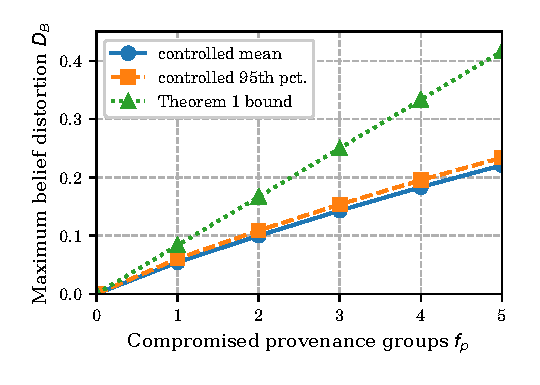
\includegraphics[width=\columnwidth]{figures/kgfedmarl_belief_budget.eps}
\caption{Controlled belief-distortion experiment under increasing numbers of compromised provenance groups. The controlled mean and 95th percentile remain below the sufficient bound from Theorem~\ref{thm-bounded-poisoning}.}
\label{fig-exp-belief-budget}
\end{figure}

The controlled mean $D_B$ increases from 0.0543 at $f_p=1$ to 0.2208 at $f_p=5$, while the corresponding 95th percentiles are 0.0605 and 0.2339. The sufficient bounds are 0.0833 and 0.4167, respectively. The gap is expected because Theorem~\ref{thm-bounded-poisoning} protects against the worst signed difference of every compromised group at every update, whereas the controlled trials sample bounded contributions within that admissible range. The important result is the scaling behavior: the implemented provenance cap keeps the empirical distortion finite and below the budget-dependent envelope as $f_p$ increases.

The correction experiment then applies the worst signed group difference for an attack lasting $H_A$ updates and removes the attack thereafter. The attacked and clean processes receive identical effective uncompromised evidence after $t_a$, matching the sufficient condition in Theorem~\ref{thm-finite-correction}. Fig.~\ref{fig-exp-correction} reports the number of updates required to return within $\epsilon_{\rm corr}=0.02$ of the reference belief.

\begin{figure}[t]
\centering
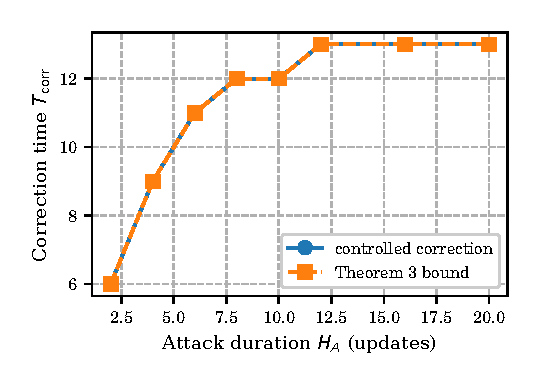
\includegraphics[width=\columnwidth]{figures/kgfedmarl_correction_time.eps}
\caption{Post-attack correction time versus poisoning duration. The controlled recurrence uses the worst per-update signed group difference and therefore follows the sufficient Theorem~\ref{thm-finite-correction} envelope closely.}
\label{fig-exp-correction}
\end{figure}

Correction requires 6 updates after a two-update attack and rises to 13 updates for the longest tested attacks. The curve saturates because the attack-induced log-odds deviation itself is bounded by the geometric accumulation in Eq.~\ref{eq-attack-duration-deviation}. This experiment also clarifies the role of forgetting: $\lambda_f$ is a security parameter, not only a tracking parameter. Increasing it preserves old evidence longer but correspondingly enlarges both the steady poisoning envelope and the post-attack correction time.

\subsection{False Authorization and Policy Propagation}
\label{subsec-exp-auth-policy}

To evaluate the semantic authorization budget, we use actions with four evidence-dependent prerequisites. The controlled belief calibration error is $\epsilon_q=0.005$ per prerequisite, and the aggregate budget $\bar\delta_B$ is swept from 0.01 to 0.10 with equal per-prerequisite allocation. For each point, 200,000 Monte Carlo actions are generated. The independence used by this generator is only an experimental convenience; Theorem~\ref{thm-false-authorization} itself uses a union bound and does not require independent prerequisites.

\begin{figure}[t]
\centering
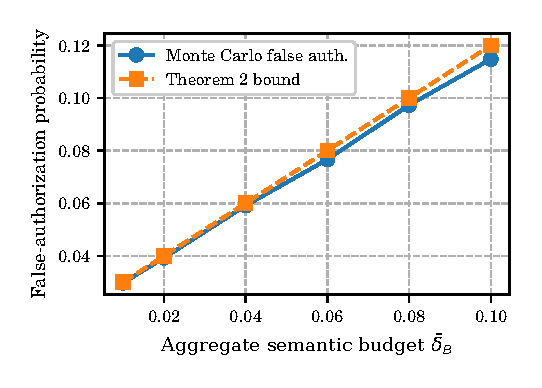
\includegraphics[width=\columnwidth]{figures/kgfedmarl_false_authorization.eps}
\caption{Controlled false-authorization probability under increasing aggregate semantic risk budget. The Monte Carlo rate remains below $\bar\delta_B+\sum_q\epsilon_q$.}
\label{fig-exp-false-auth}
\end{figure}

Across the sweep, the observed false-authorization probability ranges from 0.0297 to 0.1148, while the corresponding sufficient bounds range from 0.03 to 0.12. This experiment tests the calibration-to-authorization link rather than physical feasibility. In the complete recovery loop, a candidate that passes the semantic gate is still subject to the authoritative verifier over $\widehat{\mathcal X}_t$; consequently, the semantic risk budget cannot authorize an invariant physical violation.

The policy-propagation experiment uses 64 fixed audit states and a four-action categorical policy. The attacked and reference deployments start from the same policy and undergo up to ten successful promotion events. Candidate updates are projected to satisfy the trust-dependent KL radii $\kappa_\pi(0.55)=0.00215$ for the lower-trust attacked stream and $\kappa_\pi(0.90)=0.0032$ for the reference stream. Fig.~\ref{fig-exp-policy-drift} compares the resulting audit-distribution TV distance with the cumulative Theorem~\ref{thm-policy-drift} envelope.

\begin{figure}[t]
\centering
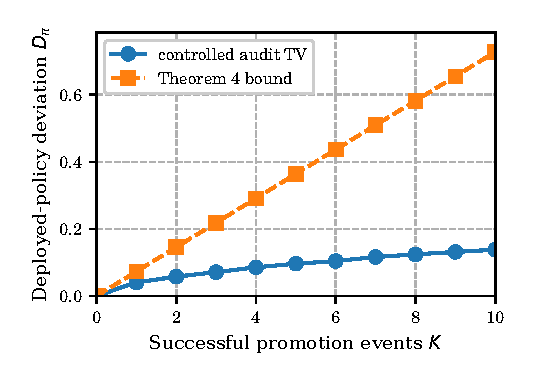
\includegraphics[width=\columnwidth]{figures/kgfedmarl_policy_drift.eps}
\caption{Controlled deployed-policy drift on a fixed audit distribution. The sufficient Theorem~\ref{thm-policy-drift} bound is intentionally conservative because it accumulates worst-case per-promotion TV changes through a triangle inequality.}
\label{fig-exp-policy-drift}
\end{figure}

After ten promotions, the controlled attacked-versus-reference policy deviation is 0.1379, whereas the sufficient cumulative bound is 0.7279. The numerical gap should not be interpreted as looseness that can be removed without stronger assumptions: the theorem deliberately avoids requiring a positive lower bound on every action probability and allows attacked and reference promotion paths to move in different directions at every event. The experiment instead demonstrates that the implemented projection and fixed-audit comparison produce policy changes that remain inside the claimed security envelope.

\subsection{Feeder-Level Recovery Protocol and Ablations}
\label{subsec-exp-feeder}

The final end-to-end study should embed the same evidence manipulation operators in the existing power-system recovery environment and should not replace them with direct policy corruption. The legacy experiment scripts already define IEEE 33-bus, 69-bus, 123-node, and 8500-node recovery layouts and conventional physical/reinforcement-learning baselines; those layouts can be retained, while the old KG/MARL/FL-centric ablations should be replaced by security-boundary ablations that match the revised paper.

The primary end-to-end comparison should include: (i) a physical optimization or rule-based restoration baseline such as MISOCP/FLISR; (ii) a decentralized MARL baseline using the same physical observations but no recovery knowledge plane; (iii) a static-KG MARL baseline that consumes graph features but treats runtime assertions as trusted; and (iv) full KG-FedMARL. The mechanism ablations should disable one trust boundary at a time: \emph{No provenance cap}, \emph{No temporal forgetting}, \emph{No semantic gate}, \emph{No transition quarantine}, and \emph{Fixed promotion radius}. These variants correspond directly to the four security objectives and are more informative for the revised paper than removing generic GAT, asynchronous FL, or personalized adapters.

For each feeder and attack class, the experiment should report mean $\pm$ standard deviation over at least five independent seeds, together with the exact $\Omega_A$, number of evidence sources, number of independent provenance groups, and number of task-critical prerequisites per action. The physical results should be presented jointly with the security metrics. In particular, a method should not be described as better merely because it restores more load if it also raises the false-authorization rate or bypasses the certified fallback more often. The recommended result tuple is
\begin{align}
\big(
\mathrm{AURC},\,
T_{\rm crit},\,
D_B,\,
P_{\rm FA},\,
T_{\rm corr},\,
D_\pi,\,
r_{\rm fb},\,
T_{\rm gate}
\big),
\end{align}
where $r_{\rm fb}$ is the fallback frequency and $T_{\rm gate}$ is the online authorization latency.

\subsection{Reproducibility and Result Provenance}
\label{subsec-exp-repro}

The script \path{figures/Code/kgfedmarl_security_experiments.py} reproduces all numerical curves reported in Figs.~\ref{fig-exp-belief-budget}--\ref{fig-exp-policy-drift} from a fixed seed. It exports vector PDF/EPS files and high-resolution PNG files and can be used as the mechanism-level regression test when the implementation changes. The earlier plotting programs in \texttt{figures/Code} remain useful as layout and baseline templates, but their hard-coded arrays are not treated as measured evidence in this revision. Before final submission, feeder-level figures should be regenerated from archived co-simulation logs or CSV files with seed-level observations, and the manuscript should report only statistics that can be traced back to those files.
\section{CONCLUSION}
This paper studied resilient restoration of power cyber-physical systems when the runtime knowledge used for recovery may itself be incomplete, stale, conflicting, replayed, or adversarially manipulated. We formulated this attack surface as \emph{recovery knowledge poisoning} and treated the recovery knowledge plane as an explicit security object rather than as trusted side information. KG-FedMARL separates a protected semantic basis from uncertain runtime assertions and limits two propagation paths: from adversarial evidence to recovery beliefs and action authority, and from contaminated recovery transitions to the deployed policy. The framework combines a provenance-aware temporal belief update with bounded source-group influence, a risk-aware recovery gate that separates uncertain semantic prerequisites from authoritative physical verification, and trust-gated online policy adaptation with quarantined replay and stable--candidate policy separation. Dynamic knowledge graphs, decentralized MARL, and federated training remain compatible implementation mechanisms, but none is assumed to provide the security guarantee by itself.

Under the stated trust boundary, the security analysis provides mechanism-level guarantees that connect the adversarial evidence budget and framework parameters to four quantities: accumulated recovery-belief distortion, false-authorization risk, post-attack belief-correction time, and cumulative deployed-policy deviation. Controlled experiments remain inside the corresponding sufficient envelopes. In the 20-seed IEEE 33-bus feeder study under medium mixed poisoning, KG-FedMARL reduces mean false authorization by 73.6\% relative to the latest-evidence baseline and by 90.0\% relative to the static-KG baseline, while its AURC remains within about 0.9\% of the oracle-information AC reference. The security ablations further separate the roles of provenance capping, forgetting, semantic authorization, and replay quarantine. On the 8500-node stress case, the conservative AC verifier rejects every additional restoration block from the configured initial state, producing a fail-safe but liveness-limited fallback regime. We report this limitation explicitly: the result supports bounded execution rather than successful large-feeder restoration and motivates feeder-aware candidate partitioning and verifier tuning.

These guarantees and experiments remain conditional on authenticated source identities, protected semantic and actuation components, correct provenance grouping and belief-update implementation, containment of the realized state in the verifier's conservative state set, and an uncompromised authoritative verifier. They do not establish global convergence of the underlying nonlinear MARL optimizer and do not cover arbitrary corruption of the trusted semantic basis, verifier code, protected actuation path, or all independent provenance groups. Within these boundaries, KG-FedMARL provides a concrete way to reason about and experimentally trace how far corrupted recovery knowledge can propagate through an online cyber-physical restoration loop.


\bibliographystyle{IEEEtran}
\bibliography{ref}

\end{document}
